\section{Combinatorial manifolds}

\begin{frame}{Manifolds in HoTT}
\begin{itemize}
\item Recall the classical theory of \alert{simplicial complexes}
\item Define a \alert{realization} procedure to construct types
\end{itemize}
\end{frame}

\begin{frame}{Simplicial complexes}
\begin{columns}
\begin{column}{0.5\textwidth}
\begin{mydef}
An \defemph{abstract simplicial complex \( M \) of dimension \( n \)} is an ordered list of sets \( M\defeq[M_0,\ldots,M_n] \) consisting of 
\begin{itemize}
\item a set \( M_0 \) of vertices
\item sets \( M_k \) of subsets of \( M_0 \) of cardinality \( k+1 \)
\item downward closed: if \( F\in M_k \) and \( G\subseteq F \), \( |G|=j+1 \) then \( G\in M_j \)
\end{itemize}
We call the truncated list \( M_{\leq k}\defeq [M_0,\ldots,M_k] \) \alert{the \( k \)-skeleton of \( M \)}.
\end{mydef}
\end{column}
\begin{column}{0.5\textwidth}
\resizebox{220pt}{!}{
\onslide<2->{
\begin{tikzpicture}
  \matrix (A) [matrix of math nodes, row sep=1cm, column sep=-.2cm]
  { M_2\\ M_1\\ M_0\\ };
\end{tikzpicture}
\begin{tikzpicture}
    \matrix (A) [matrix of math nodes, row sep=1cm, column sep=-.2cm]
    { 
  ~ &  ~ & \scriptstyle\{w, b, r\} & \scriptstyle\{w, r, g\}  & \scriptstyle\{w, g, o\} & \scriptstyle\{w, o, b\} & \scriptstyle\{y, b, r\} & \scriptstyle\{y, r, g\}  & \scriptstyle\{y, g, o\} & \scriptstyle\{y, o, b\}\\
  \scriptstyle\{w, b\} & \scriptstyle\{w,r\}  & \scriptstyle\{w,g\} & \scriptstyle\{w,o\} & \scriptstyle\{b, r\} & \scriptstyle\{r, g\}  & \scriptstyle\{g, o\} & \scriptstyle\{o, b\} & \scriptstyle\{y, b\} & \scriptstyle\{y,r\}  & \scriptstyle\{y,g\} & \scriptstyle\{y,o\}\\
  ~ & ~ & ~ &  \scriptstyle w  & \scriptstyle b & \scriptstyle r & \scriptstyle g & \scriptstyle o & \scriptstyle y\\
    };

    \draw (A-1-3.south)--(A-2-1.north);
    \draw (A-1-3.south)--(A-2-2.north);
    \draw (A-1-3.south)--(A-2-5.north);

    \draw (A-1-4.south)--(A-2-2.north);
    \draw (A-1-4.south)--(A-2-3.north);
    \draw (A-1-4.south)--(A-2-6.north);

    \draw (A-1-5.south)--(A-2-3.north);
    \draw (A-1-5.south)--(A-2-4.north);
    \draw (A-1-5.south)--(A-2-7.north);

    \draw (A-1-6.south)--(A-2-4.north);
    \draw (A-1-6.south)--(A-2-1.north);
    \draw (A-1-6.south)--(A-2-8.north);

    \draw (A-1-7.south)--(A-2-5.north);
    \draw (A-1-7.south)--(A-2-10.north);
    \draw (A-1-7.south)--(A-2-9.north);

    \draw (A-1-8.south)--(A-2-6.north);
    \draw (A-1-8.south)--(A-2-11.north);
    \draw (A-1-8.south)--(A-2-10.north);

    \draw (A-1-9.south)--(A-2-7.north);
    \draw (A-1-9.south)--(A-2-12.north);
    \draw (A-1-9.south)--(A-2-11.north);

    \draw (A-1-10.south)--(A-2-8.north);
    \draw (A-1-10.south)--(A-2-9.north);
    \draw (A-1-10.south)--(A-2-12.north);

    \draw (A-2-1.south)--(A-3-4.north);
    \draw (A-2-1.south)--(A-3-5.north);

    \draw (A-2-2.south)--(A-3-4.north);
    \draw (A-2-2.south)--(A-3-6.north);

    \draw (A-2-3.south)--(A-3-4.north);
    \draw (A-2-3.south)--(A-3-7.north);

    \draw (A-2-4.south)--(A-3-4.north);
    \draw (A-2-4.south)--(A-3-8.north);

    \draw (A-2-5.south)--(A-3-5.north);
    \draw (A-2-5.south)--(A-3-6.north);

    \draw (A-2-6.south)--(A-3-6.north);
    \draw (A-2-6.south)--(A-3-7.north);

    \draw (A-2-7.south)--(A-3-7.north);
    \draw (A-2-7.south)--(A-3-8.north);

    \draw (A-2-8.south)--(A-3-8.north);
    \draw (A-2-8.south)--(A-3-5.north);

    \draw (A-2-9.south)--(A-3-9.north);
    \draw (A-2-9.south)--(A-3-5.north);

    \draw (A-2-10.south)--(A-3-9.north);
    \draw (A-2-10.south)--(A-3-6.north);

    \draw (A-2-11.south)--(A-3-9.north);
    \draw (A-2-11.south)--(A-3-7.north);

    \draw (A-2-12.south)--(A-3-9.north);
    \draw (A-2-12.south)--(A-3-8.north);
\end{tikzpicture}
}
}
\onslide<2->{\begin{figure}[h]
\centering
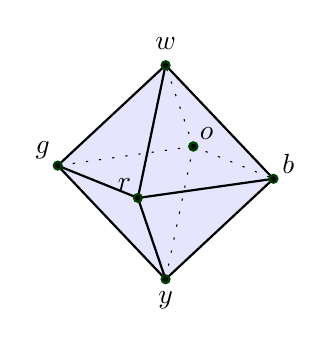
\begin{tikzpicture}%
  [x={(-0.860769cm, -0.121512cm)},
  y={(0.508996cm, -0.205391cm)},
  z={(-0.000053cm, 0.971107cm)},
  scale=1,
  back/.style={loosely dotted, thin},
  edge/.style={black, thick},
  facet/.style={fill=blue!95!black,fill opacity=0.1},
  vertex/.style={inner sep=1pt,circle,draw=green!25!black,fill=black,thick}]
\coordinate (-1, -1, 0) at (-1, -1, 0);
\coordinate (-1, 1, 0) at (-1, 1, 0);
\coordinate (0, 0, -1) at (0, 0, -1);
\coordinate (0, 0, 1) at (0, 0, 1);
\coordinate (1, -1, 0) at (1, -1, 0);
\coordinate (1, 1, 0) at (1, 1, 0);
%% Drawing edges in the back
%%
\draw[edge,back] (-1, -1, 0) -- (-1, 1, 0);
\draw[edge,back] (-1, -1, 0) -- (0, 0, -1.4);
\draw[edge,back] (-1, -1, 0) -- (0, 0, 1.4);
\draw[edge,back] (-1, -1, 0) -- (1, -1, 0);
%% Drawing vertices in the back
%%
\node[vertex] at (-1, -1, 0)     {};
%% Drawing the facets
%%
\fill[facet] (1, 1, 0) -- (0, 0, -1.4) -- (1, -1, 0) -- cycle {};
\fill[facet] (1, 1, 0) -- (0, 0, 1.4) -- (1, -1, 0) -- cycle {};
\fill[facet] (1, 1, 0) -- (-1, 1, 0) -- (0, 0, 1.4) -- cycle {};
\fill[facet] (1, 1, 0) -- (-1, 1, 0) -- (0, 0, -1.4) -- cycle {};
%% Drawing edges in the front
%%
\draw[edge] (-1, 1, 0) -- (0, 0, -1.4);
\draw[edge] (-1, 1, 0) -- (0, 0, 1.4);
\draw[edge] (-1, 1, 0) -- (1, 1, 0);
\draw[edge] (0, 0, -1.4) -- (1, -1, 0);
\draw[edge] (0, 0, -1.4) -- (1, 1, 0);
\draw[edge] (0, 0, 1.4) -- (1, -1, 0);
\draw[edge] (0, 0, 1.4) -- (1, 1, 0);
\draw[edge] (1, -1, 0) -- (1, 1, 0);
%% Drawing the vertices in the front
%%
\begin{scope}[nodes=vertex]
\node[label=above right:\( b \)] at (-1, 1, 0)     {};
\node[label=below:\( y \)] at (0, 0, -1.4)     {};
\node[label=above:\( w \)] at (0, 0, 1.4)     {};
\node[label=above left:\( g \)] at (1, -1, 0)     {};
\node[label=above left:\( r \)] at (1, 1, 0)     {};
\node[label=above right:\( o \)] at (-1, -1, 0)     {};
\end{scope}
\end{tikzpicture}
\caption{The HIT \( \oo \) which has 6 points, 12 1-paths, 8 2-paths.}
\end{figure}
}
\onslide<2->{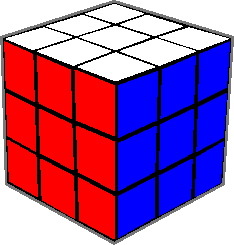
\includegraphics[width=60pt]{figs/hungarian_cube.pdf}}
\end{column}
\end{columns}
\end{frame}

\begin{frame}{Simplicial complexes}
\begin{example}
The \defemph{complete simplex of dimension \( n \)}, denoted \alert{\( \Delta(n), \)} is the set \( \{0,\ldots,n\} \) and its power set. The \( (n-1) \)-skeleton \( \Delta(n)_{\leq (n-1)} \) is denoted \alert{\( \partial \Delta(n) \)} and will serve as a combinatorial \( (n-1) \)-sphere.
\end{example}
\( \Delta(1) \) is visually 
\begin{tikzpicture}[baseline=-1.2mm]
\tikzset{oo/.style={circle, scale=0.25, fill=black}}
\node[oo, label=left:\( 0 \)] at (-0.7, 0) (a) {};
\node[oo, label=right:\( 1 \)] at  (0.7, 0) (c) {};
\draw[fill=blue!95!black,fill opacity=0.1] (-0.7, 0)--(0.7, 0);
\end{tikzpicture}, 
\( \partial\Delta(1) \) is visually
\begin{tikzpicture}[baseline=-1.2mm]
\tikzset{oo/.style={circle, scale=0.25, fill=black}}
\node[oo, label=left:\( 0 \)] at (-0.7, 0) (a) {};
\node[oo, label=right:\( 1 \)] at  (0.7, 0) (c) {};
\end{tikzpicture}, 

\( \Delta(2) \) is visually 
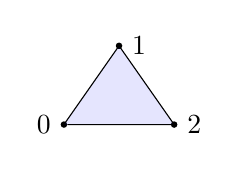
\begin{tikzpicture}[baseline=3mm]
\tikzset{oo/.style={circle, scale=0.25, fill=black}}
\node[oo, label=left:\( 0 \)] at (-0.7, 0) (a) {};
\node[oo, label=right:\( 1 \)] at  (0, 1) (b) {};
\node[oo, label=right:\( 2 \)] at  (0.7, 0) (c) {};
\draw[fill=blue!95!black,fill opacity=0.1] (-0.7, 0)--(0, 1)--(0.7, 0)--(a);
\end{tikzpicture}, 
\( \partial \Delta(2) \) is visually 
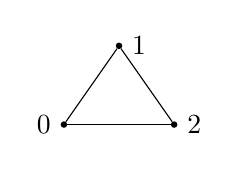
\begin{tikzpicture}[baseline=3mm]
\tikzset{oo/.style={circle, scale=0.25, fill=black}}
\node[oo, label=left:\( 0 \)] at (-0.7, 0) (a) {};
\node[oo, label=right:\( 1 \)] at  (0, 1) (b) {};
\node[oo, label=right:\( 2 \)] at  (0.7, 0) (c) {};
\draw (a) -- (b);
\draw (b) -- (c);
\draw (c) -- (a);
\end{tikzpicture}
\end{frame}

\begin{frame}{Homotopy realization: dimension 0}
We will \alert{realize} simplicial complexes by means of \alert{a sequence of pushouts}.

Base case: the realization \( \mm \) of a 0-dimensional complex \( M \) is \( M_0 \).

In particular the 0-sphere \( \partial\Dd(1)\defeq \partial \Delta(1)_0 \).
\end{frame}

\begin{frame}{Homotopy realization: dimension 1}
For a 1-dim complex \( M\defeq [M_0,M_1] \) the realization is given by
\[% https://q.uiver.app/#q=WzAsNCxbMCwxLCJNXzA9XFxtYXRoYmJ7TX1fMCJdLFsxLDEsIlxcbWF0aGJie019XzEiXSxbMSwwLCJNXzEiXSxbMCwwLCJNXzFcXHRpbWVzIFxcYmRzaW1wbGV4bnsxfSJdLFswLDFdLFszLDAsIlxcbWF0aGJie0F9XzAiLDJdLFszLDIsIlxcbWF0aHJte3ByfV8xIl0sWzIsMSwiKl97XFxtYXRoYmJ7TX1fMX0iXSxbMSwzLCIiLDIseyJvZmZzZXQiOjMsInN0eWxlIjp7Im5hbWUiOiJjb3JuZXItaW52ZXJzZSJ9fV0sWzAsMiwiaF8xIiwyLHsic2hvcnRlbiI6eyJzb3VyY2UiOjQwLCJ0YXJnZXQiOjQwfSwibGV2ZWwiOjJ9XV0=
\begin{tikzcd}
  {M_1\times \partial\Dd(1)} & {M_1} \\
  {M_0=\mathbb{M}_0} & {\mathbb{M}_1}
  \arrow["{\mathrm{pr}_1}", from=1-1, to=1-2]
  \arrow["{\mathbb{A}_0}"', from=1-1, to=2-1]
  \arrow["{*_{\mathbb{M}_1}}", from=1-2, to=2-2]
  \arrow["{h_1}"', shorten <=14pt, shorten >=14pt, Rightarrow, from=2-1, to=1-2]
  \arrow[from=2-1, to=2-2]
  \arrow["\ulcorner"{pos=0, rotate=180}, shift left=1, draw=none, from=2-2, to=1-1]
\end{tikzcd}
\]
\end{frame}

\begin{frame}{Homotopy realization: dimension 1}
For example the simplicial 1-sphere \( \partial\Dd(2)\defeq \)
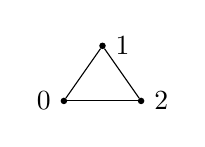
\begin{tikzpicture}[baseline=3mm, scale=0.7]
\tikzset{oo/.style={circle, scale=0.25, fill=black}}
\node[oo, label=left:\( 0 \)] at (-0.7, 0) (a) {};
\node[oo, label=right:\( 1 \)] at  (0, 1) (b) {};
\node[oo, label=right:\( 2 \)] at  (0.7, 0) (c) {};
\draw (a) -- (b);
\draw (b) -- (c);
\draw (c) -- (a);
\end{tikzpicture} is given by
\vspace{3ex}
\begin{columns}
\begin{column}{0.4\textwidth}
% https://q.uiver.app/#q=WzAsNCxbMSwwLCJcXHBhcnRpYWwgXFxEZWx0YSgyKV8xIl0sWzEsMSwiXFxwYXJ0aWFsXFxEZCgyKSJdLFswLDAsIlxccGFydGlhbCBcXERlbHRhKDIpXzFcXHRpbWVzIFxccGFydGlhbFxcRGQoMSkiXSxbMCwxLCJcXHBhcnRpYWwgXFxEZWx0YSgyKV8wIl0sWzIsMF0sWzIsM10sWzMsMV0sWzAsMV0sWzEsMiwiIiwxLHsic3R5bGUiOnsibmFtZSI6ImNvcm5lci1pbnZlcnNlIn19XSxbMywwLCJoXzEiLDIseyJzaG9ydGVuIjp7InNvdXJjZSI6MzAsInRhcmdldCI6MzB9LCJsZXZlbCI6Mn1dXQ==
\begin{tikzcd}[ampersand replacement=\&]
  {\partial \Delta(2)_1\times \partial\Dd(1)} \& {\partial \Delta(2)_1} \\
  {\partial \Delta(2)_0} \& {\partial\Dd(2)}
  \arrow[from=1-1, to=1-2]
  \arrow[from=1-1, to=2-1]
  \arrow[from=1-2, to=2-2]
  \arrow["{h_1}"', shorten <=11pt, shorten >=11pt, Rightarrow, from=2-1, to=1-2]
  \arrow[from=2-1, to=2-2]
  \arrow["\ulcorner"{pos=0, rotate=180}, draw=none, from=2-2, to=1-1]
\end{tikzcd}
\end{column}
\begin{column}{0.05\textwidth}
i.e.
\end{column}
\begin{column}{0.6\textwidth}
% https://q.uiver.app/#q=WzAsNCxbMSwwLCJcXHNjcmlwdHN0eWxlXFx7XFx7MCwgMVxcfSwgXFx7MSwgMlxcfSwgXFx7MiwgMFxcfVxcfSJdLFsxLDEsIlxccGFydGlhbFxcRGQoMikiXSxbMCwwLCJcXHNjcmlwdHN0eWxlXFx7XFx7MCwgMVxcfSwgXFx7MSwgMlxcfSwgXFx7MiwgMFxcfVxcfVxcdGltZXMgXFx7MCwgMVxcfSJdLFswLDEsIlxcc2NyaXB0c3R5bGVcXHswLCAxLCAyXFx9Il0sWzIsMF0sWzIsM10sWzMsMV0sWzAsMV0sWzEsMiwiIiwxLHsic3R5bGUiOnsibmFtZSI6ImNvcm5lci1pbnZlcnNlIn19XSxbMywwLCJoXzEiLDIseyJzaG9ydGVuIjp7InNvdXJjZSI6MzAsInRhcmdldCI6MzB9LCJsZXZlbCI6Mn1dXQ==
\begin{tikzcd}[ampersand replacement=\&]
  {\scriptstyle\{\{0, 1\}, \{1, 2\}, \{2, 0\}\}\times \{0, 1\}} \& {\scriptstyle\{\{0, 1\}, \{1, 2\}, \{2, 0\}\}} \\
  {\scriptstyle\{0, 1, 2\}} \& {\partial\Dd(2)}
  \arrow[from=1-1, to=1-2]
  \arrow[from=1-1, to=2-1]
  \arrow[from=1-2, to=2-2]
  \arrow["{h_1}"', shorten <=13pt, shorten >=13pt, Rightarrow, from=2-1, to=1-2]
  \arrow[from=2-1, to=2-2]
  \arrow["\ulcorner"{pos=0, rotate=180}, draw=none, from=2-2, to=1-1]
\end{tikzcd}
\end{column}
\end{columns}
\end{frame}

\begin{frame}{Homotopy realization: dimension 1}
Or the 1-skeleton of the octahedron \( \oo \):
% https://q.uiver.app/#q=WzAsNCxbMCwxLCJcXHt3LCBnLFxcbGRvdHNcXH0iXSxbMCwwLCJcXHtcXHt3LCBnXFx9LFxcbGRvdHNcXH1cXHRpbWVzXFx7MCwxXFx9Il0sWzEsMCwiXFx7XFx7dyxnXFx9LFxcbGRvdHNcXH0iXSxbMSwxLCJcXG9vXzEiXSxbMSwyXSxbMSwwXSxbMCwzXSxbMiwzXSxbMywxLCIiLDEseyJzdHlsZSI6eyJuYW1lIjoiY29ybmVyLWludmVyc2UifX1dLFswLDIsImhfMSIsMix7InNob3J0ZW4iOnsic291cmNlIjozMCwidGFyZ2V0IjozMH0sImxldmVsIjoyfV1d
\[\begin{tikzcd}[ampersand replacement=\&]
  {\{\{w, g\},\ldots\}\times\{0,1\}} \& {\{\{w,g\},\ldots\}} \\
  {\{w, g,\ldots\}} \& {\oo_1}
  \arrow[from=1-1, to=1-2]
  \arrow[from=1-1, to=2-1]
  \arrow[from=1-2, to=2-2]
  \arrow["{h_1}"', shorten <=11pt, shorten >=11pt, Rightarrow, from=2-1, to=1-2]
  \arrow[from=2-1, to=2-2]
  \arrow["\ulcorner"{anchor=center, pos=0.125, rotate=180}, draw=none, from=2-2, to=1-1]
\end{tikzcd}\]
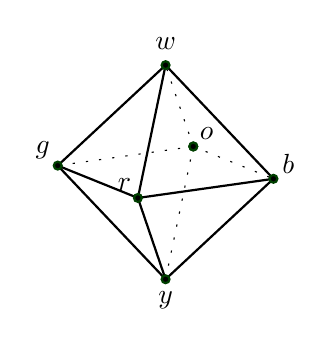
\begin{tikzpicture}%
  [x={(-0.860769cm, -0.121512cm)},
  y={(0.508996cm, -0.205391cm)},
  z={(-0.000053cm, 0.971107cm)},
  scale=1,
  back/.style={loosely dotted, thin},
  edge/.style={black, thick},
  facet/.style={fill=blue!95!black,fill opacity=0.0},
  vertex/.style={inner sep=1pt,circle,draw=green!25!black,fill=black,thick}]
\coordinate (-1, -1, 0) at (-1, -1, 0);
\coordinate (-1, 1, 0) at (-1, 1, 0);
\coordinate (0, 0, -1) at (0, 0, -1);
\coordinate (0, 0, 1) at (0, 0, 1);
\coordinate (1, -1, 0) at (1, -1, 0);
\coordinate (1, 1, 0) at (1, 1, 0);
%% Drawing edges in the back
%%
\draw[edge,back] (-1, -1, 0) -- (-1, 1, 0);
\draw[edge,back] (-1, -1, 0) -- (0, 0, -1.4);
\draw[edge,back] (-1, -1, 0) -- (0, 0, 1.4);
\draw[edge,back] (-1, -1, 0) -- (1, -1, 0);
%% Drawing vertices in the back
%%
\node[vertex] at (-1, -1, 0)     {};
%% Drawing the facets
%%
\fill[facet] (1, 1, 0) -- (0, 0, -1.4) -- (1, -1, 0) -- cycle {};
\fill[facet] (1, 1, 0) -- (0, 0, 1.4) -- (1, -1, 0) -- cycle {};
\fill[facet] (1, 1, 0) -- (-1, 1, 0) -- (0, 0, 1.4) -- cycle {};
\fill[facet] (1, 1, 0) -- (-1, 1, 0) -- (0, 0, -1.4) -- cycle {};
%% Drawing edges in the front
%%
\draw[edge] (-1, 1, 0) -- (0, 0, -1.4);
\draw[edge] (-1, 1, 0) -- (0, 0, 1.4);
\draw[edge] (-1, 1, 0) -- (1, 1, 0);
\draw[edge] (0, 0, -1.4) -- (1, -1, 0);
\draw[edge] (0, 0, -1.4) -- (1, 1, 0);
\draw[edge] (0, 0, 1.4) -- (1, -1, 0);
\draw[edge] (0, 0, 1.4) -- (1, 1, 0);
\draw[edge] (1, -1, 0) -- (1, 1, 0);
%% Drawing the vertices in the front
%%
\begin{scope}[nodes=vertex]
\node[label=above right:\( b \)] at (-1, 1, 0)     {};
\node[label=below:\( y \)] at (0, 0, -1.4)     {};
\node[label=above:\( w \)] at (0, 0, 1.4)     {};
\node[label=above left:\( g \)] at (1, -1, 0)     {};
\node[label=above left:\( r \)] at (1, 1, 0)     {};
\node[label=above right:\( o \)] at (-1, -1, 0)     {};
\end{scope}
\end{tikzpicture}

\end{frame}

\begin{frame}{Homotopy realization: dimension 2}
To realize \( M\defeq[M_0, M_1, M_2] \) use \(  \partial\Dd(1), \partial\Dd(2) \):
\[% https://q.uiver.app/#q=WzAsNyxbMCwwLCJNXzFcXHRpbWVzIFxccGFydGlhbFxcRGQoMSkiXSxbMCwxLCJNXzA9XFxtYXRoYmJ7TX1fMCJdLFsxLDEsIlxcbWF0aGJie019XzEiXSxbMSwwLCJNXzEiXSxbMSwyLCJNXzJcXHRpbWVzIFxccGFydGlhbFxcRGQoMikiXSxbMiwyLCJNXzIiXSxbMiwxLCJcXG1hdGhiYntNfV8yIl0sWzAsMSwiXFxtYXRoYmJ7QX1fMCIsMl0sWzEsMl0sWzAsMywiXFxtYXRocm17cHJ9XzEiXSxbMywyLCIqX3tcXG1hdGhiYntNfV8xfSJdLFsyLDAsIiIsMSx7InN0eWxlIjp7Im5hbWUiOiJjb3JuZXItaW52ZXJzZSJ9fV0sWzIsNl0sWzQsMiwiXFxtYXRoYmJ7QX1fMSJdLFs1LDYsIipfe1xcbWF0aGJie019XzJ9IiwyXSxbNCw1LCJcXG1hdGhybXtwcn1fMSIsMl0sWzYsNCwiIiwxLHsic3R5bGUiOnsibmFtZSI6ImNvcm5lci1pbnZlcnNlIn19XSxbMiw1LCJoXzIiLDAseyJzaG9ydGVuIjp7InNvdXJjZSI6NDAsInRhcmdldCI6NDB9LCJsZXZlbCI6Mn1dLFsxLDMsImhfMSIsMix7InNob3J0ZW4iOnsic291cmNlIjo0MCwidGFyZ2V0Ijo0MH0sImxldmVsIjoyfV1d
\begin{tikzcd}[ampersand replacement=\&]
  {M_1\times \partial\Dd(1)} \& {M_1} \\
  {M_0=\mathbb{M}_0} \& {\mathbb{M}_1} \& {\mathbb{M}_2} \\
  \& {M_2\times \partial\Dd(2)} \& {M_2}
  \arrow["{\mathrm{pr}_1}", from=1-1, to=1-2]
  \arrow["{\mathbb{A}_0}"', from=1-1, to=2-1]
  \arrow["{*_{\mathbb{M}_1}}", from=1-2, to=2-2]
  \arrow["{h_1}"', shorten <=17pt, shorten >=17pt, Rightarrow, from=2-1, to=1-2]
  \arrow[from=2-1, to=2-2]
  \arrow["\ulcorner"{anchor=center, pos=0.125, rotate=180}, draw=none, from=2-2, to=1-1]
  \arrow[from=2-2, to=2-3]
  \arrow["{h_2}", shorten <=13pt, shorten >=13pt, Rightarrow, from=2-2, to=3-3]
  \arrow["\ulcorner"{anchor=center, pos=0.125, rotate=-90}, draw=none, from=2-3, to=3-2]
  \arrow["{\mathbb{A}_1}", from=3-2, to=2-2]
  \arrow["{\mathrm{pr}_1}"', from=3-2, to=3-3]
  \arrow["{*_{\mathbb{M}_2}}"', from=3-3, to=2-3]
\end{tikzcd}
\]
\end{frame}

\begin{frame}{Homotopy realization: dimension 2}
The full octahedron \( \oo \):
\begin{columns}
\begin{column}{0.75\textwidth}
% https://q.uiver.app/#q=WzAsNyxbMCwwLCJcXHtcXHt3LCBnXFx9LFxcbGRvdHNcXH1cXHRpbWVzXFx7MCwxXFx9Il0sWzAsMSwiXFx7dywgZyxcXGxkb3RzXFx9Il0sWzEsMSwiXFxvb18xIl0sWzEsMCwiXFx7XFx7dyxnXFx9LFxcbGRvdHNcXH0iXSxbMSwyLCJcXHtcXHt3LGcsclxcfSxcXGxkb3RzXFx9XFx0aW1lcyBcXHBhcnRpYWxcXERkKDIpIl0sWzIsMiwiXFx7XFx7dyxnLHJcXH0sXFxsZG90c1xcfSJdLFsyLDEsIlxcb29fMiJdLFswLDFdLFsxLDJdLFswLDMsIlxcbWF0aHJte3ByfV8xIl0sWzMsMl0sWzIsMCwiIiwxLHsic3R5bGUiOnsibmFtZSI6ImNvcm5lci1pbnZlcnNlIn19XSxbMiw2XSxbNCwyXSxbNSw2XSxbNCw1LCJcXG1hdGhybXtwcn1fMSIsMl0sWzYsNCwiIiwxLHsic3R5bGUiOnsibmFtZSI6ImNvcm5lci1pbnZlcnNlIn19XSxbMiw1LCJoXzIiLDAseyJzaG9ydGVuIjp7InNvdXJjZSI6NDAsInRhcmdldCI6NDB9LCJsZXZlbCI6Mn1dLFsxLDMsImhfMSIsMix7InNob3J0ZW4iOnsic291cmNlIjo0MCwidGFyZ2V0Ijo0MH0sImxldmVsIjoyfV1d
\[\begin{tikzcd}[ampersand replacement=\&, column sep=small]
  {\{\{w, g\},\ldots\}\times\{0,1\}} \& {\{\{w,g\},\ldots\}} \\
  {\{w, g,\ldots\}} \& {\oo_1} \& {\oo_2} \\
  \& {\{\{w,g,r\},\ldots\}\times \partial\Dd(2)} \& {\{\{w,g,r\},\ldots\}}
  \arrow["{\mathrm{pr}_1}", from=1-1, to=1-2]
  \arrow[from=1-1, to=2-1]
  \arrow[from=1-2, to=2-2]
  \arrow["{h_1}"', shorten <=22pt, shorten >=22pt, Rightarrow, from=2-1, to=1-2]
  \arrow[from=2-1, to=2-2]
  \arrow["\ulcorner"{pos=0.05, rotate=180}, draw=none, from=2-2, to=1-1]
  \arrow[from=2-2, to=2-3]
  \arrow["{h_2}", shorten <=21pt, shorten >=21pt, Rightarrow, from=2-2, to=3-3]
  \arrow["\ulcorner"{pos=-0.1, rotate=-90}, draw=none, from=2-3, to=3-2]
  \arrow[from=3-2, to=2-2]
  \arrow["{\mathrm{pr}_1}"', from=3-2, to=3-3]
  \arrow[from=3-3, to=2-3]
\end{tikzcd}\]
\end{column}
\begin{column}{0.25\textwidth}
\begin{figure}[h]
\centering
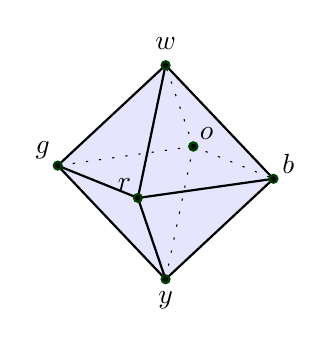
\begin{tikzpicture}%
  [x={(-0.860769cm, -0.121512cm)},
  y={(0.508996cm, -0.205391cm)},
  z={(-0.000053cm, 0.971107cm)},
  scale=1,
  back/.style={loosely dotted, thin},
  edge/.style={black, thick},
  facet/.style={fill=blue!95!black,fill opacity=0.1},
  vertex/.style={inner sep=1pt,circle,draw=green!25!black,fill=black,thick}]
\coordinate (-1, -1, 0) at (-1, -1, 0);
\coordinate (-1, 1, 0) at (-1, 1, 0);
\coordinate (0, 0, -1) at (0, 0, -1);
\coordinate (0, 0, 1) at (0, 0, 1);
\coordinate (1, -1, 0) at (1, -1, 0);
\coordinate (1, 1, 0) at (1, 1, 0);
%% Drawing edges in the back
%%
\draw[edge,back] (-1, -1, 0) -- (-1, 1, 0);
\draw[edge,back] (-1, -1, 0) -- (0, 0, -1.4);
\draw[edge,back] (-1, -1, 0) -- (0, 0, 1.4);
\draw[edge,back] (-1, -1, 0) -- (1, -1, 0);
%% Drawing vertices in the back
%%
\node[vertex] at (-1, -1, 0)     {};
%% Drawing the facets
%%
\fill[facet] (1, 1, 0) -- (0, 0, -1.4) -- (1, -1, 0) -- cycle {};
\fill[facet] (1, 1, 0) -- (0, 0, 1.4) -- (1, -1, 0) -- cycle {};
\fill[facet] (1, 1, 0) -- (-1, 1, 0) -- (0, 0, 1.4) -- cycle {};
\fill[facet] (1, 1, 0) -- (-1, 1, 0) -- (0, 0, -1.4) -- cycle {};
%% Drawing edges in the front
%%
\draw[edge] (-1, 1, 0) -- (0, 0, -1.4);
\draw[edge] (-1, 1, 0) -- (0, 0, 1.4);
\draw[edge] (-1, 1, 0) -- (1, 1, 0);
\draw[edge] (0, 0, -1.4) -- (1, -1, 0);
\draw[edge] (0, 0, -1.4) -- (1, 1, 0);
\draw[edge] (0, 0, 1.4) -- (1, -1, 0);
\draw[edge] (0, 0, 1.4) -- (1, 1, 0);
\draw[edge] (1, -1, 0) -- (1, 1, 0);
%% Drawing the vertices in the front
%%
\begin{scope}[nodes=vertex]
\node[label=above right:\( b \)] at (-1, 1, 0)     {};
\node[label=below:\( y \)] at (0, 0, -1.4)     {};
\node[label=above:\( w \)] at (0, 0, 1.4)     {};
\node[label=above left:\( g \)] at (1, -1, 0)     {};
\node[label=above left:\( r \)] at (1, 1, 0)     {};
\node[label=above right:\( o \)] at (-1, -1, 0)     {};
\end{scope}
\end{tikzpicture}
\caption{The HIT \( \oo \) which has 6 points, 12 1-paths, 8 2-paths.}
\end{figure}

\end{column}
\end{columns}
\end{frame}

\begin{frame}{Homotopy realization: dimension 2}
\begin{columns}
\begin{column}{0.25\textwidth}
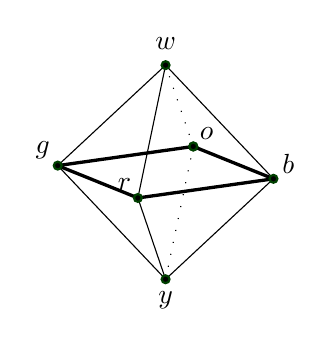
\begin{tikzpicture}%
  [x={(-0.860769cm, -0.121512cm)},
  y={(0.508996cm, -0.205391cm)},
  z={(-0.000053cm, 0.971107cm)},
  scale=1,
  eqback/.style={very thick},
  back/.style={loosely dotted, thin},
  eqedge/.style={very thick},
  edge/.style={black, thin},
  r/.style={},
  facet/.style={fill=blue!95!black,fill opacity=0.0},
  vertex/.style={inner sep=1pt,circle,draw=green!25!black,fill=black,thick}]
\coordinate (-1, -1, 0) at (-1, -1, 0);
\coordinate (-1, 1, 0) at (-1, 1, 0);
\coordinate (0, 0, -1) at (0, 0, -1);
\coordinate (0, 0, 1) at (0, 0, 1);
\coordinate (1, -1, 0) at (1, -1, 0);
\coordinate (1, 1, 0) at (1, 1, 0);
%% Drawing edges in the back
%%
\draw[edge,eqback] (-1, -1, 0) -- (-1, 1, 0);
\draw[edge,back] (-1, -1, 0) -- (0, 0, -1.4);
\draw[edge,back] (-1, -1, 0) -- (0, 0, 1.4);
\draw[edge,eqback] (1, -1, 0) -- (-1, -1, 0);
%% Drawing vertices in the back
%%
\node[vertex] at (-1, -1, 0)     {};
%% Drawing the facets
%%
%\fill[facet] (1, 1, 0) -- (0, 0, -1.4) -- (1, -1, 0) -- cycle {};
%\fill[facet] (1, 1, 0) -- (0, 0, 1.4) -- (1, -1, 0) -- cycle {};
\fill[facet] (1, 1, 0) -- (-1, 1, 0) -- (0, 0, 1.4) -- cycle {};
%\fill[facet] (1, 1, 0) -- (-1, 1, 0) -- (0, 0, -1.4) -- cycle {};
%% Drawing edges in the front
%%
\draw[edge] (-1, 1, 0) -- (0, 0, -1.4);
\draw[edge] (-1, 1, 0) -- (0, 0, 1.4);
\draw[eqedge] (-1, 1, 0) -- (1, 1, 0);
\draw[edge] (0, 0, -1.4) -- (1, -1, 0);
\draw[edge] (0, 0, -1.4) -- (1, 1, 0);
\draw[edge] (0, 0, 1.4) -- (1, -1, 0);
\draw[edge] (0, 0, 1.4) -- (1, 1, 0);
\draw[r,eqedge] (1, 1, 0) -- (1, -1, 0);
%% Drawing the vertices in the front
%%
\begin{scope}[nodes=vertex]
\node[label=above right:\( b \)] at (-1, 1, 0)     {};
\node[label=below:\( y \)] at (0, 0, -1.4)     {};
\node[label=above:\( w \)] at (0, 0, 1.4)     {};
\node[label=above left:\( g \)] at (1, -1, 0)     {};
\node[label=above left:\( r \)] at (1, 1, 0)     {};
\node[label=above right:\( o \)] at (-1, -1, 0)     {};
\end{scope}
\end{tikzpicture}

\end{column}
\begin{column}{0.15\textwidth}
\( \leftarrow\link(w) \)
\end{column}
\begin{column}{0.6\textwidth}
The \defemph{link} of a vertex \( w \) in a 2-complex is: the sets not containing \( w \) but whose union with \( w \) is a face.\\~\\

A \alert{combinatorial manifold} is a simplicial complex all of whose links are\( ^* \) simplicial spheres.\\~\\

This will be our model of the \alert{tangent space}.\\~\\
\end{column}
\end{columns}
\vspace{5ex}
{\scriptsize\( {}^* \)the (classical) geometric realization is homeomorphic to a sphere}
\end{frame}

\begin{frame}{Combinatorial manifolds \( \leftrightarrow \) smooth manifolds}
\begin{theorem}[Whitehead (1940)]
Every smooth \( n \)-manifold has a compatible structure of a \alert{combinatorial manifold}: a simplicial complex of dimension \( n \) such that the link is a combinatorial \( (n-1) \)-sphere, i.e. its geometric realization is an \( (n-1) \)-sphere.
\end{theorem}
\url{https://ncatlab.org/nlab/show/triangulation+theorem}

\onslide<2->{Counterexample: Wikipedia says this is a simplicial complex, but we can see it fails the link condition:

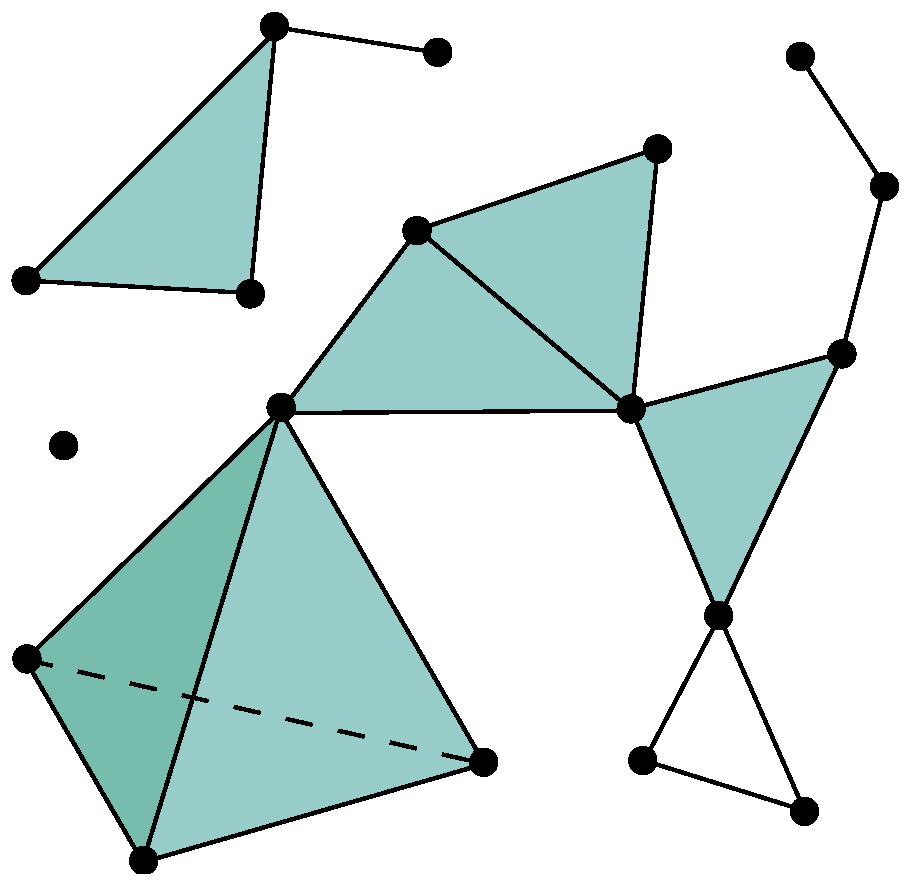
\includegraphics[width=15ex]{figs/simplicial_complex_example.pdf}}
\end{frame}

